%% LaTeX Beamer presentation template (requires beamer package)
%% see http://bitbucket.org/rivanvx/beamer/wiki/Home
%% idea contributed by H. Turgut Uyar
%% template based on a template by Till Tantau
%% this template is still evolving - it might differ in future releases!

% \documentclass[handout]{beamer}
\documentclass{beamer}

\mode<presentation>
{
% \usetheme{Rochester}
% \usecolortheme{seahorse}
% \usetheme{Antibes}
% \usecolortheme{dolphin}
% \usetheme{Hannover}
% \usecolortheme{whale}
\usetheme{Pittsburgh}
\usecolortheme{seahorse}
\setbeamercovered{transparent}
}

\usepackage[english]{babel}
\usepackage[latin1]{inputenc}

% font definitions, try \usepackage{ae} instead of the following
% three lines if you don't like this look
\usepackage{mathptmx}
\usepackage[scaled=.90]{helvet}
\usepackage{courier}
\usepackage{tabulary}


\usepackage[T1]{fontenc}


\title{Introduction to source control with git}

%\subtitle{}

% - Use the \inst{?} command only if the authors have different
%   affiliation.
\author{Sam Procter}
% \author{\inst{1}}

% - Use the \inst command only if there are several affiliations.
% - Keep it simple, no one is interested in your street address.
\institute{Department of Computing and Information Sciences\\
Kansas State University}

\date{Tuesday, September 16, 2014}


% This is only inserted into the PDF information catalog. Can be left
% out.
\subject{Talks}



% If you have a file called "university-logo-filename.xxx", where xxx
% is a graphic format that can be processed by latex or pdflatex,
% resp., then you can add a logo as follows:

% \pgfdeclareimage[height=0.5cm]{university-logo}{university-logo-filename}
% \logo{\pgfuseimage{university-logo}}



% Delete this, if you do not want the table of contents to pop up at
% the beginning of each subsection:
\AtBeginSubsection[]
{
\begin{frame}<beamer>
\frametitle{Outline}
\tableofcontents[currentsection,currentsubsection]
\end{frame}
}

% If you wish to uncover everything in a step-wise fashion, uncomment
% the following command:

%\beamerdefaultoverlayspecification{<+->}

\begin{document}

\begin{frame}
\titlepage
\end{frame}

\begin{frame}
\frametitle{Before we begin}
\begin{enumerate}
  \uncover<1->{\item I'm not a git expert}
  \begin{itemize}
    \uncover<2->{\item But I use git \emph{every} day at my job}
  \end{itemize} 
  \uncover<3->{\item You can learn how to use git on your own}
  \begin{itemize}
    \uncover<4->{\item I'll show you a basic introduction and give you an
    \emph{understanding} of git}
  \end{itemize}
  \uncover<5->{\item Follow along at:
  \alert{http://people.cis.ksu.edu/\textasciitilde samprocter/git-intro.pdf}}
\end{enumerate}
\end{frame}


\begin{frame}
\frametitle{Outline}
\tableofcontents
% You might wish to add the option [pausesections]
\end{frame}


\section{Source Control Management}

\subsection[Why Source Control?]{Why use source control?}

\begin{frame}
\frametitle{Why use source control?}
\uncover<1->{How do you share projects now?}

\uncover<2->{What happens if\ldots}

\begin{itemize}
  \uncover<3->{\item You delete some code but realize later that you need it?}
  \uncover<4->{\item You do some work on a lab machine, and then want to work on
  your pc at home?}
  \uncover<5->{\item Your laptop dies?}
  \uncover<6->{\item Two people change the same file?}
\end{itemize}
\uncover<7->{Solution: Source Control!}

\end{frame}

\subsection[Source Control History]{A history of Source Control Tools}

\begin{frame}
\frametitle{A super-brief history of source control}
\begin{table}
\scriptsize
\centering
\begin{tabulary}{\textwidth}{l|l|l|L|L}
Gen. & Networking & Operations & Concurrency & Examples \\\hline
1 & None & One file at a time & Locks & SCCS\\
2 & Centralized & Multi-file & Merge before commit & CVS, SVN\\
3 & Distributed & Changesets & Commit before merge & git, hg
\end{tabulary}
\caption{Source control through the years, adapted from \cite{sink:BOOK2011}}
\end{table}
\begin{enumerate}
  \uncover<1->{\item SCCS: 1972, File locks, no sharing at all}
  \uncover<2->{\item CVS, SVN: 1986 (CVS), deltas, merging}
  \uncover<3->{\item git, Mercurial: 2005, "file system snapshots" distributed}
\end{enumerate}
\end{frame}

\section{git}
\subsection[Git Background]{Git Background}
\begin{frame}
\frametitle{Where did git come from?}
\framesubtitle{``Git began with a bit of creative destruction and fiery
controversy''\cite{sink:BOOK2011}}
\begin{figure}[!t] \centering

\includegraphics[width=.3\textwidth]{figures/git}
\end{figure}
Git was created by Linus Torvalds (and other Linux developers) with aims of:
\begin{itemize}
  \uncover<1->{\item Speed}
  \uncover<1->{\item Simplicity}
  \uncover<1->{\item Distributivity}
\end{itemize}
\end{frame}

\begin{frame}
\frametitle{Git Concepts}
% \framesubtitle{``Git began with a bit of creative destruction and fiery
% controversy''\cite{sink:BOOK2011}}

\begin{figure}[!t] \centering
\only<1|handout:1>{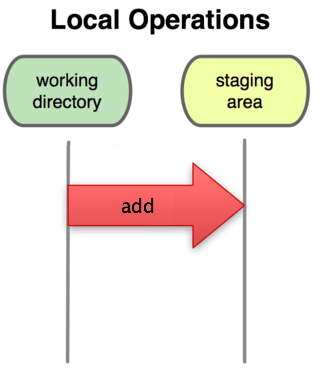
\includegraphics[width=.3\textwidth]{figures/staging-area}}
\only<2|handout:2>{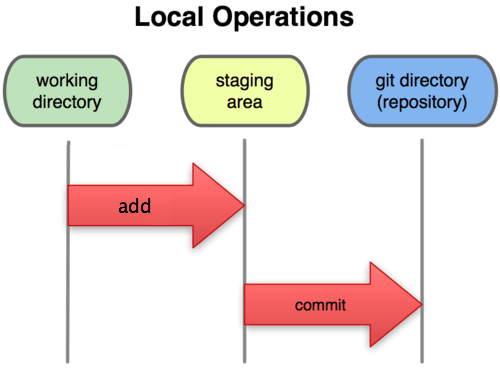
\includegraphics[width=.4\textwidth]{figures/local-operations}}
\only<3|handout:3>{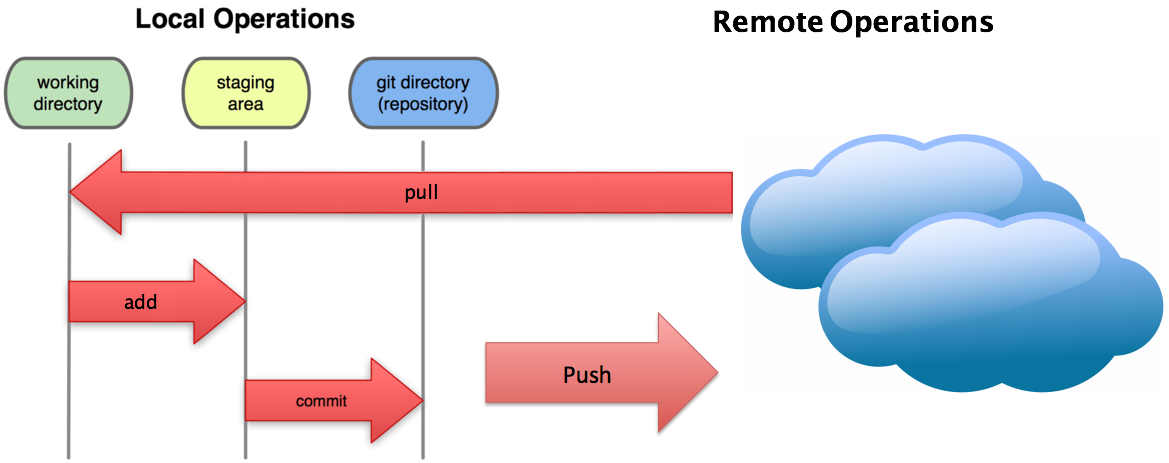
\includegraphics[width=.8\textwidth]{figures/full-diagram}}
\end{figure}
\begin{itemize}
  \uncover<1->{\item Working Directory: Your modified files}
  \uncover<1->{\item Staging Area: Files To be shipped with the next commit}
  \uncover<2->{\item Git Directory: The official record}
  \uncover<3->{\item The cloud: github, \textasciitilde yourname, etc.}
\end{itemize}
\end{frame}

\subsection[Getting and making changes]{Getting and making changes}

\begin{frame}
\frametitle{Sharing changes with git commit \& push}
\alert{Situation:} You've created three files -- a.txt, b.txt, and c.txt. You
want to share a.txt and b.txt, but \emph{not} c.txt.

\vspace{.05\textwidth}

\uncover<2->{\alert{Strategy:} Use \texttt{git add} on a.txt and b.txt.}

\vspace{.05\textwidth}

\begin{enumerate}
  \uncover<3->{\item \texttt{\$ git add a.txt b.txt}}
  \uncover<4->{\item \texttt{\$ git commit -m 'Two new files!'}}
  \uncover<5->{\item \texttt{\$ git push}}
\end{enumerate}
\end{frame}

\begin{frame}
\frametitle{Sharing changes quickly}
\alert{Situation:} You've changed files, but they're already tracked by git.

\vspace{.05\textwidth}

\uncover<2->{\alert{Strategy:} Use \texttt{git commit} with the \texttt{-a}
flag to add everything automatically}

\vspace{.05\textwidth}
\begin{enumerate}
  \uncover<3->{\item \texttt{\$ git commit -a -m 'Changed things'}}
  \uncover<4->{\item \texttt{\$ git push}}
\end{enumerate}
\end{frame}

\begin{frame}
\frametitle{Getting changes}
\alert{Situation:} You made changes at school, now you want to get those at
home.

\vspace{.05\textwidth}

\uncover<2->{\alert{Strategy:} Use \texttt{git pull} to get the latest version
of your files}

\vspace{.05\textwidth}
\begin{enumerate}
  \uncover<3->{\item \texttt{\$ git pull}}
\end{enumerate}
\end{frame}


\subsection[Getting a Repository]{Getting a Repostiory}

\begin{frame}
\frametitle{Git Init -- You have files}
\alert{Situation:} You've created some files, but never stored them in git.

\vspace{.05\textwidth}

\uncover<2->{\alert{Strategy:} Use \texttt{git init} to create a repository,
and \texttt{git push} to share it}

\vspace{.05\textwidth}
\begin{enumerate}
  \uncover<3->{\item \texttt{\$ git init}}
  \uncover<4->{\item \texttt{\$ git add .}}
  \uncover<5->{\item \texttt{\$ git commit -m 'First commit'}}
  \uncover<6->{\item \texttt{\$ git remote add origin <remote repo URL>}}
  \uncover<7->{\item \texttt{\$ git push origin master}}
\end{enumerate}
\uncover<3->{(Adapted from \cite{github-help})}
% \uncover<8->{Don't want to use github?  Check out
% http://support.cis.ksu.edu/UserGuide/VersionControl}
\end{frame}

\begin{frame}
\frametitle{Git Clone -- You need files}
\alert{Situation:} Files you want are on github, and you've never downloaded
them before.

\vspace{.05\textwidth}

\uncover<2->{\alert{Strategy:} Use \texttt{git clone} to get the files for the
first time}

\vspace{.05\textwidth}
\begin{enumerate}
  \uncover<3->{\item \texttt{\$ git clone <remote repo URL>}}
\end{enumerate}
\end{frame}

\subsection[Github]{Software Engineering with Github}

\begin{frame}
\frametitle{What is github?}

\begin{figure}[!t] \centering

\includegraphics[width=.4\textwidth]{figures/octocat}
\end{figure}

Github is a \alert{free*} git host.

\uncover<2->{* Free means:}
\begin{itemize}
  \uncover<3->{\item Infinite ($\infty$!) publically-accessible repositories}
  \uncover<4->{\item Five free private repositories for students}
\end{itemize}
\end{frame}

\begin{frame}
\frametitle{Using github}

\begin{figure}[!t] \centering
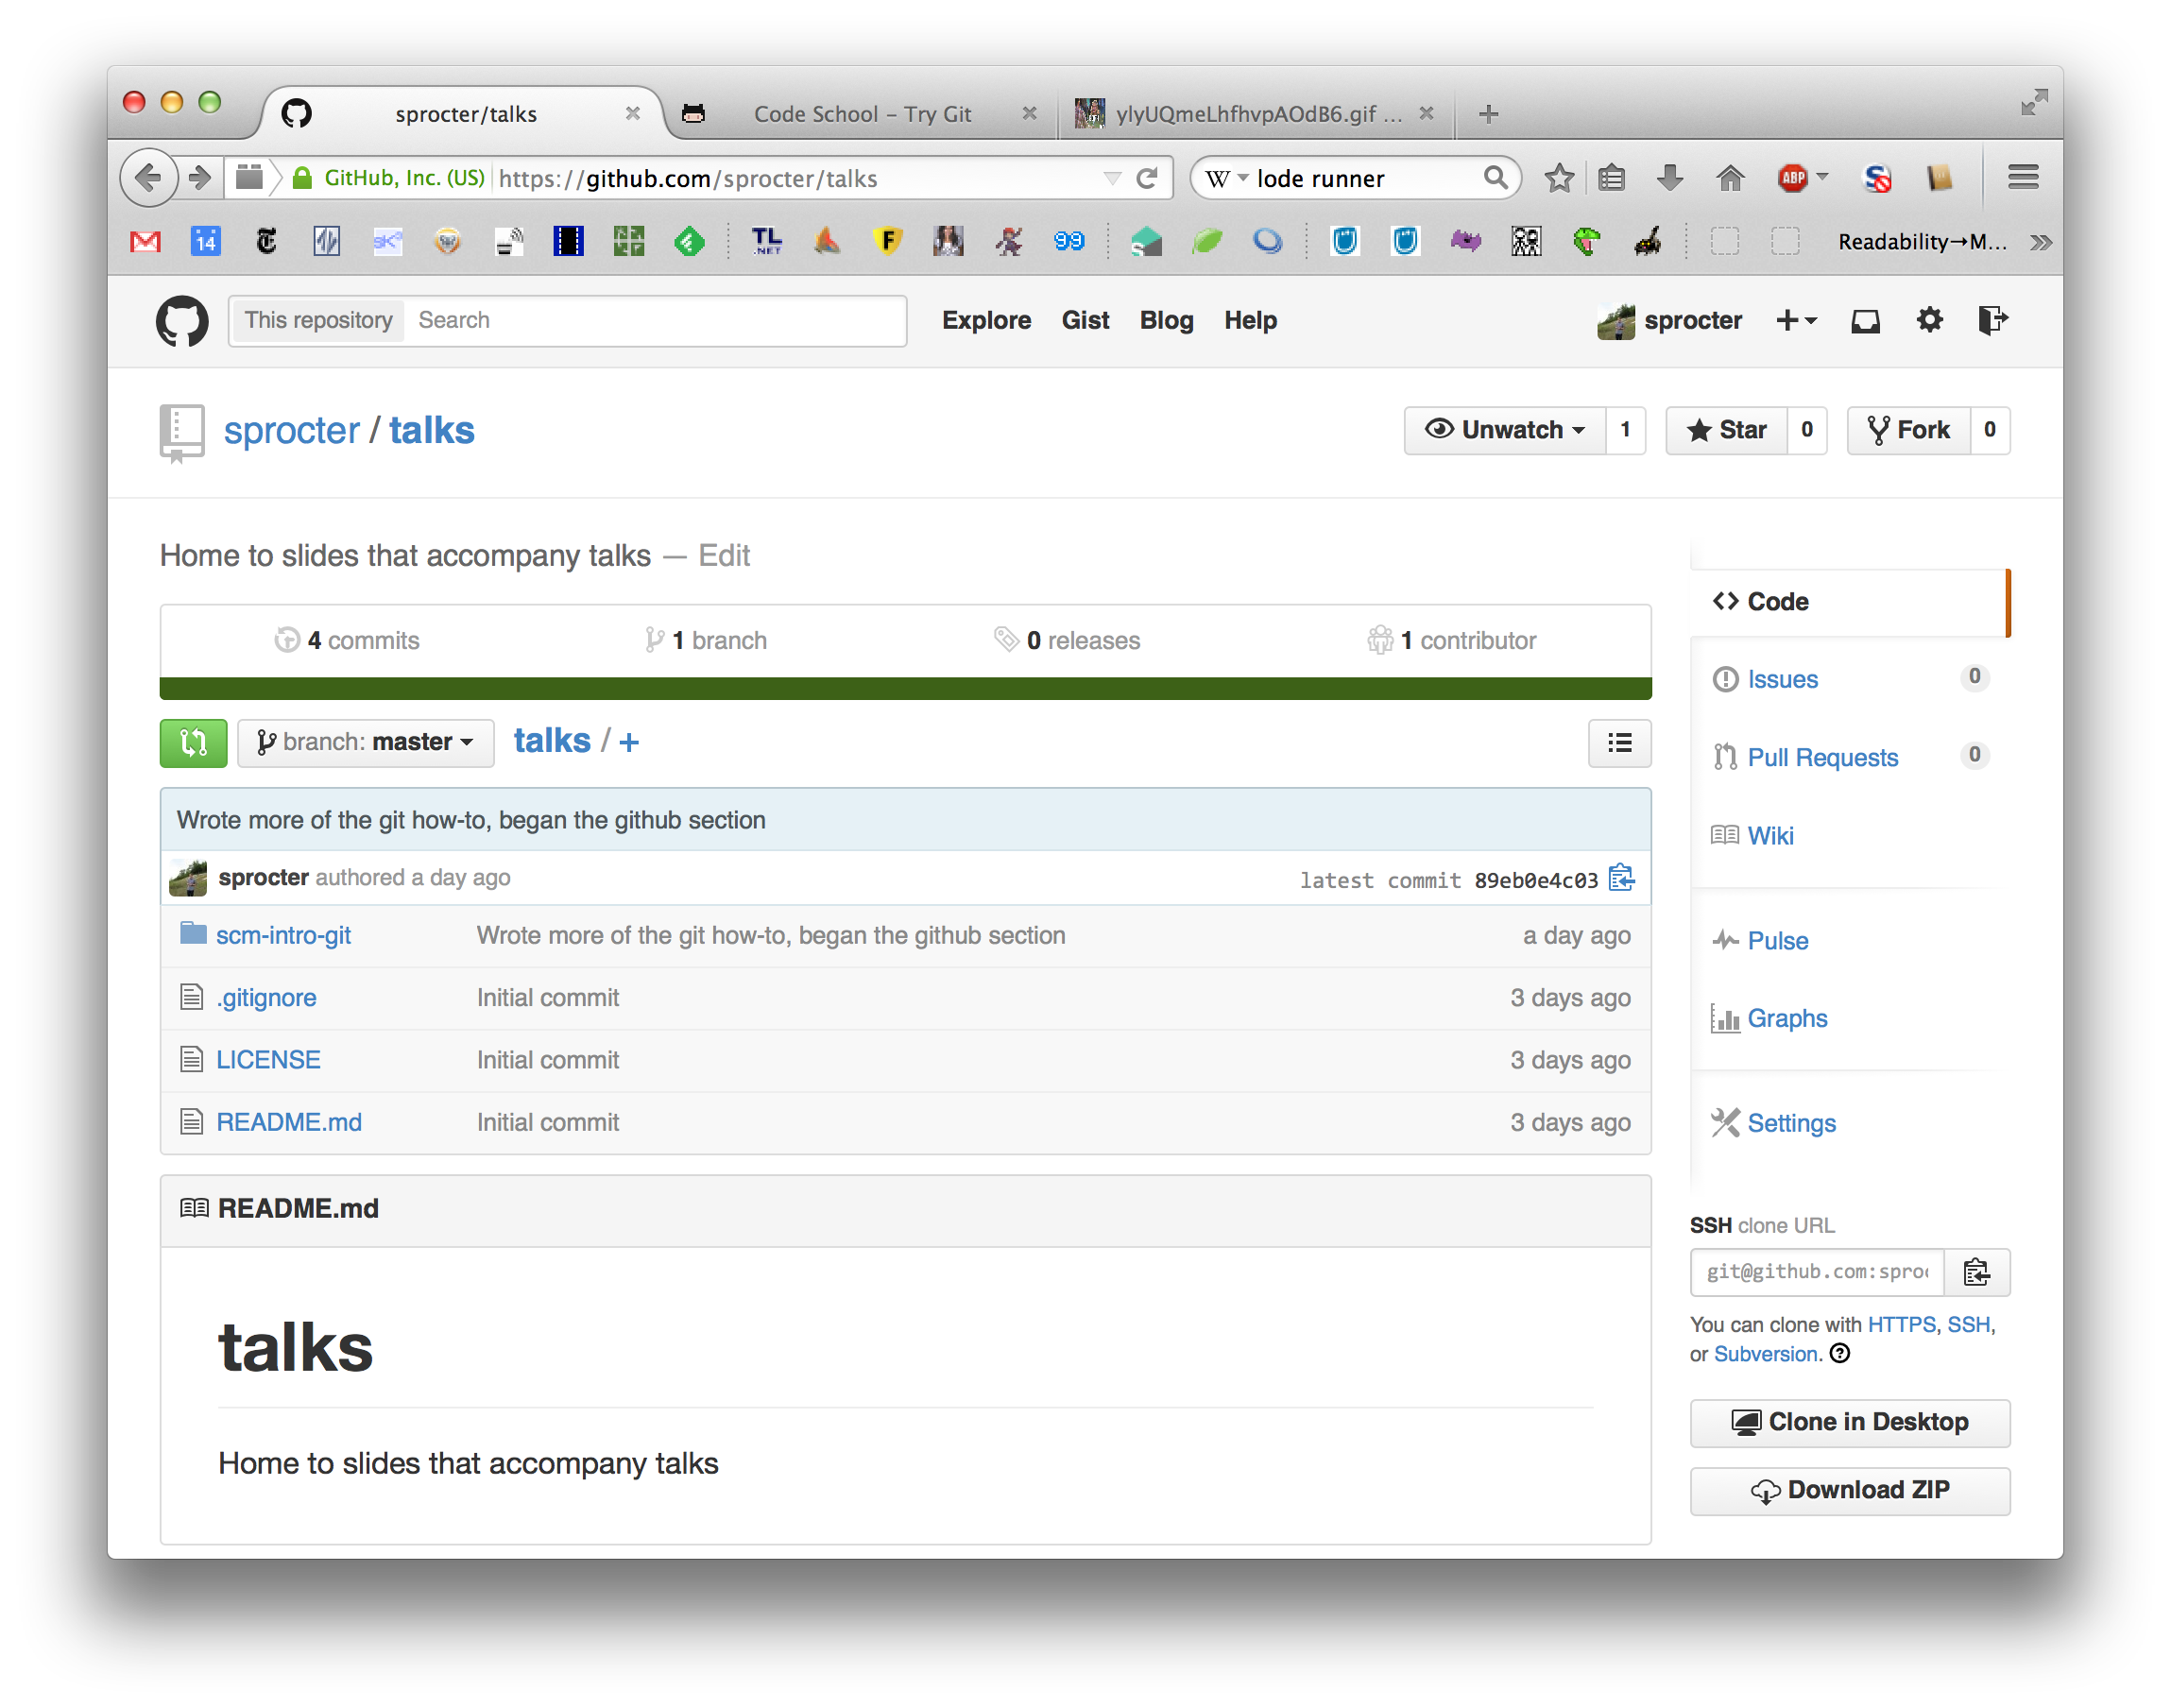
\includegraphics[width=.8\textwidth]{figures/github-home}
\end{figure}

\end{frame}

\begin{frame}
\frametitle{Viewing the list of commits}

\begin{figure}[!t] \centering
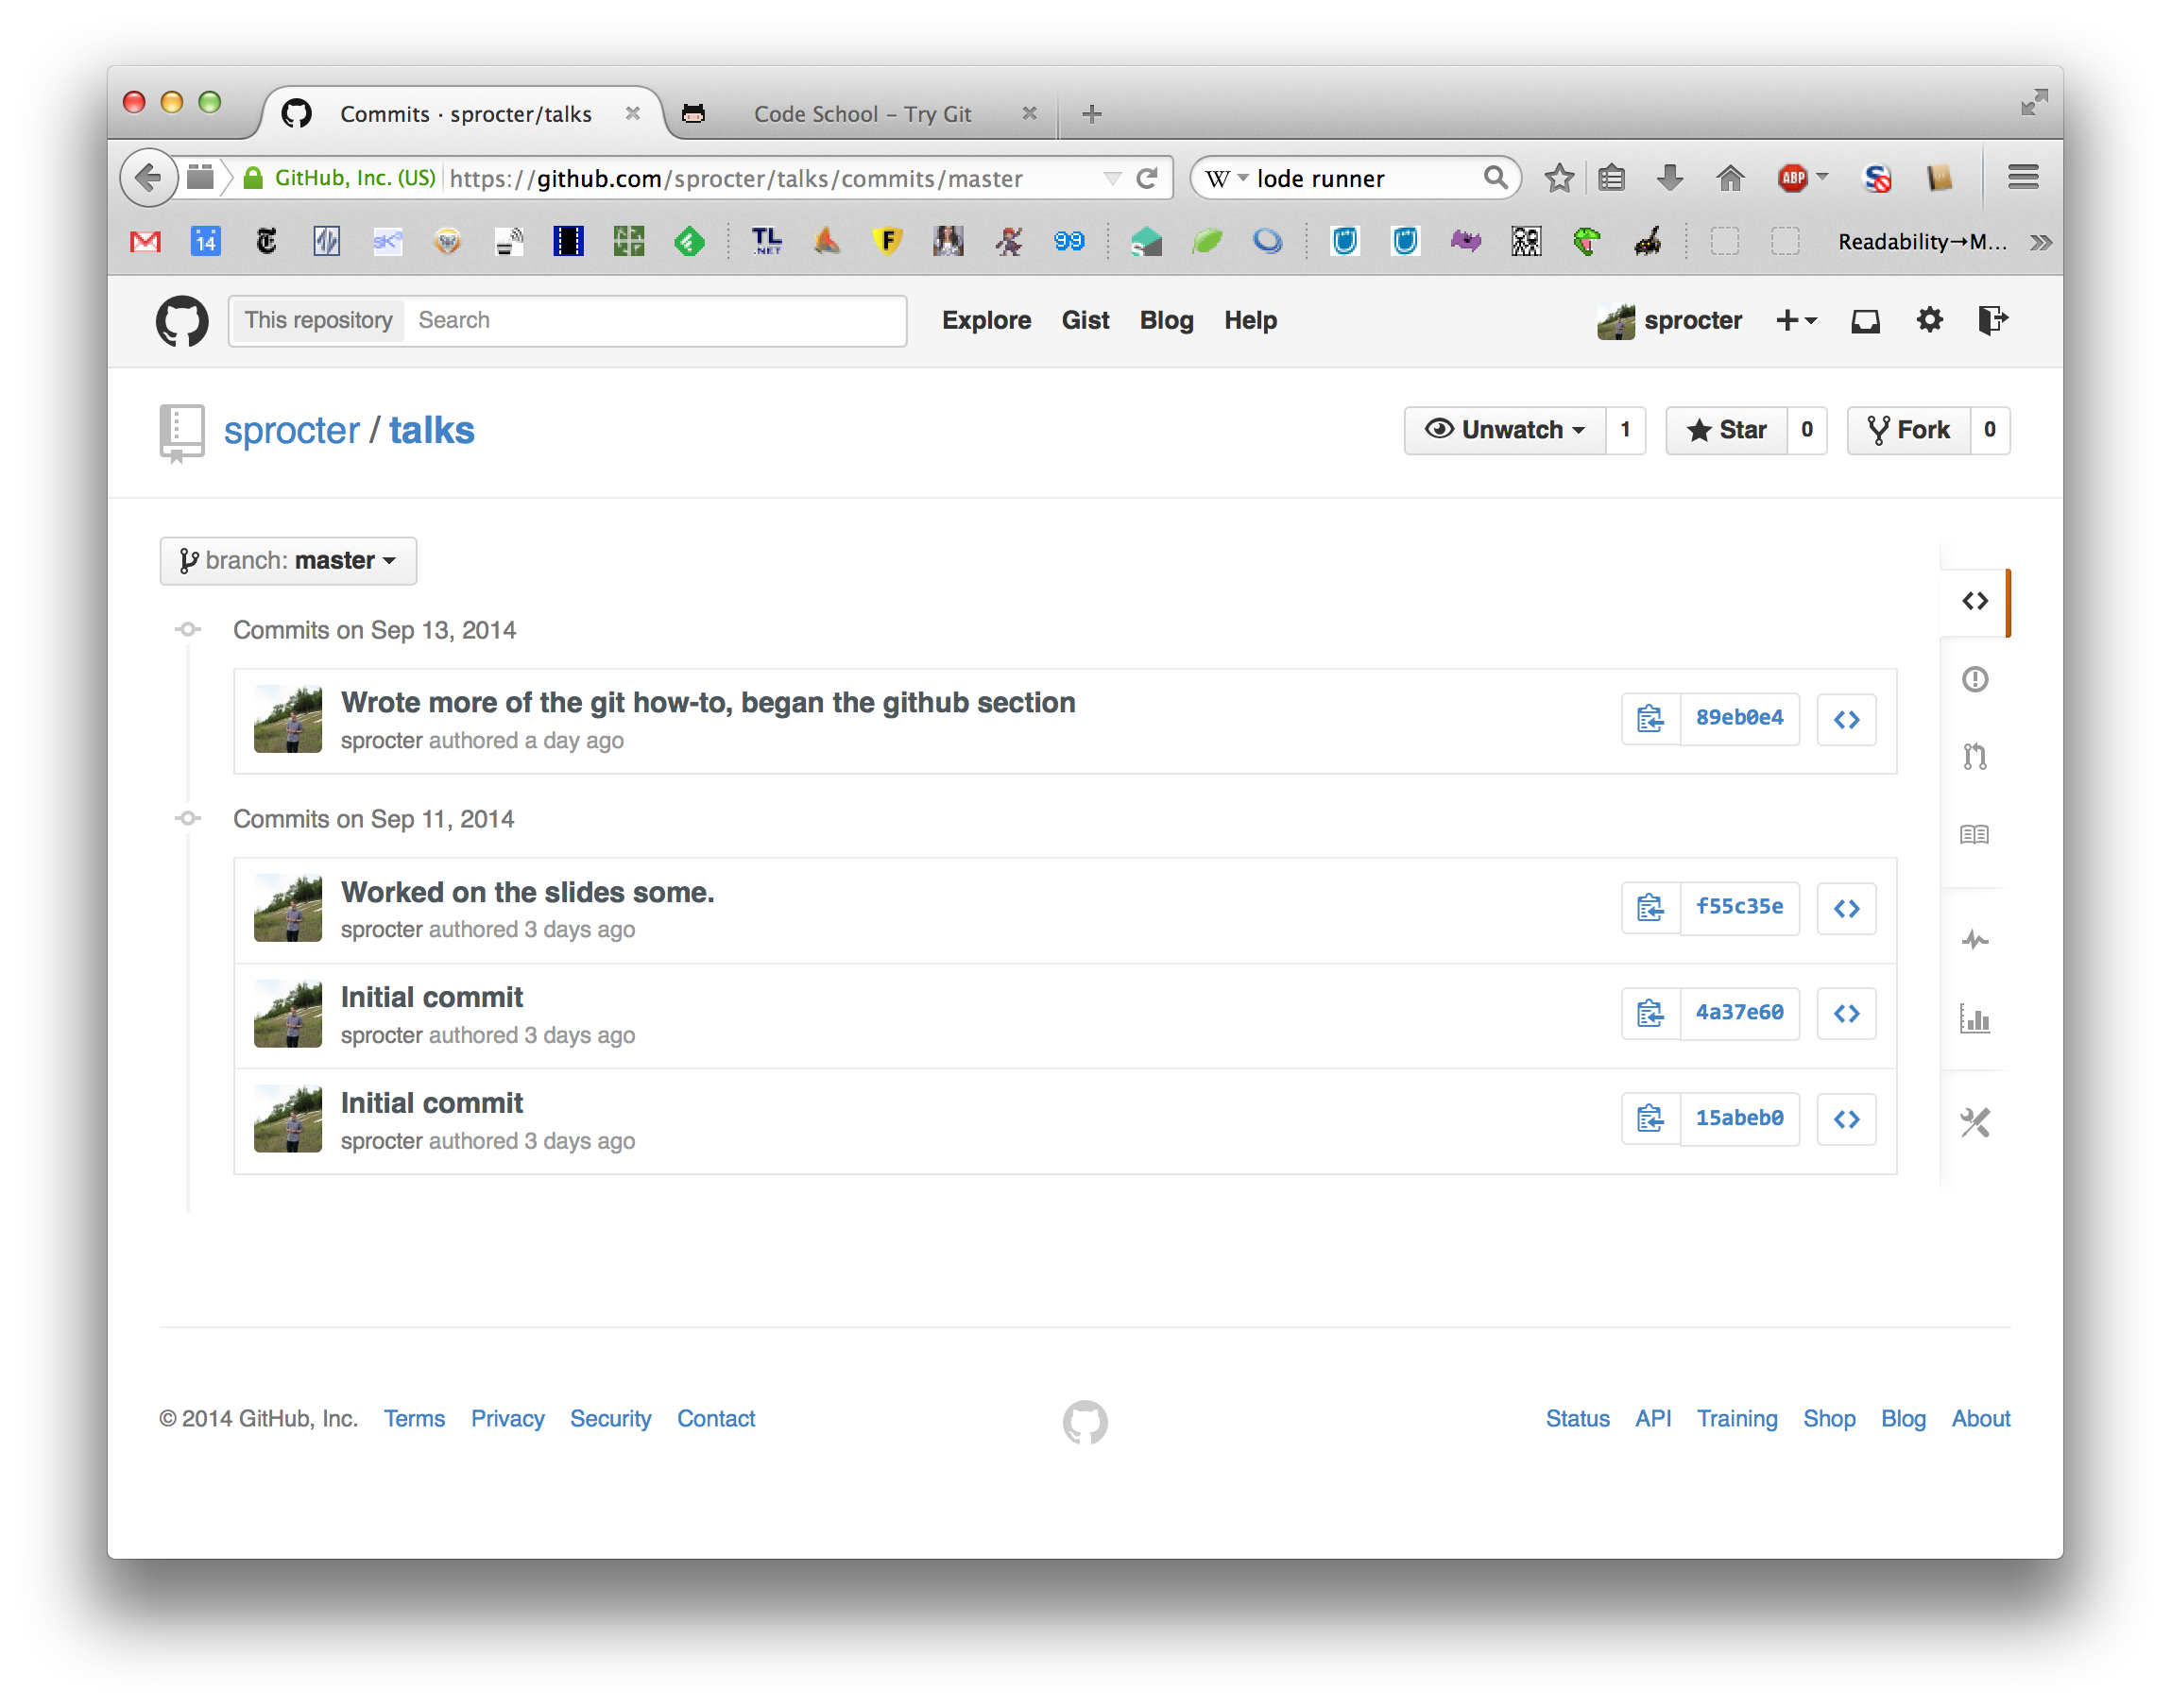
\includegraphics[width=.8\textwidth]{figures/commit-history}
\end{figure}

\end{frame}

\begin{frame}
\frametitle{Viewing the details of a commit}

\begin{figure}[!t] \centering
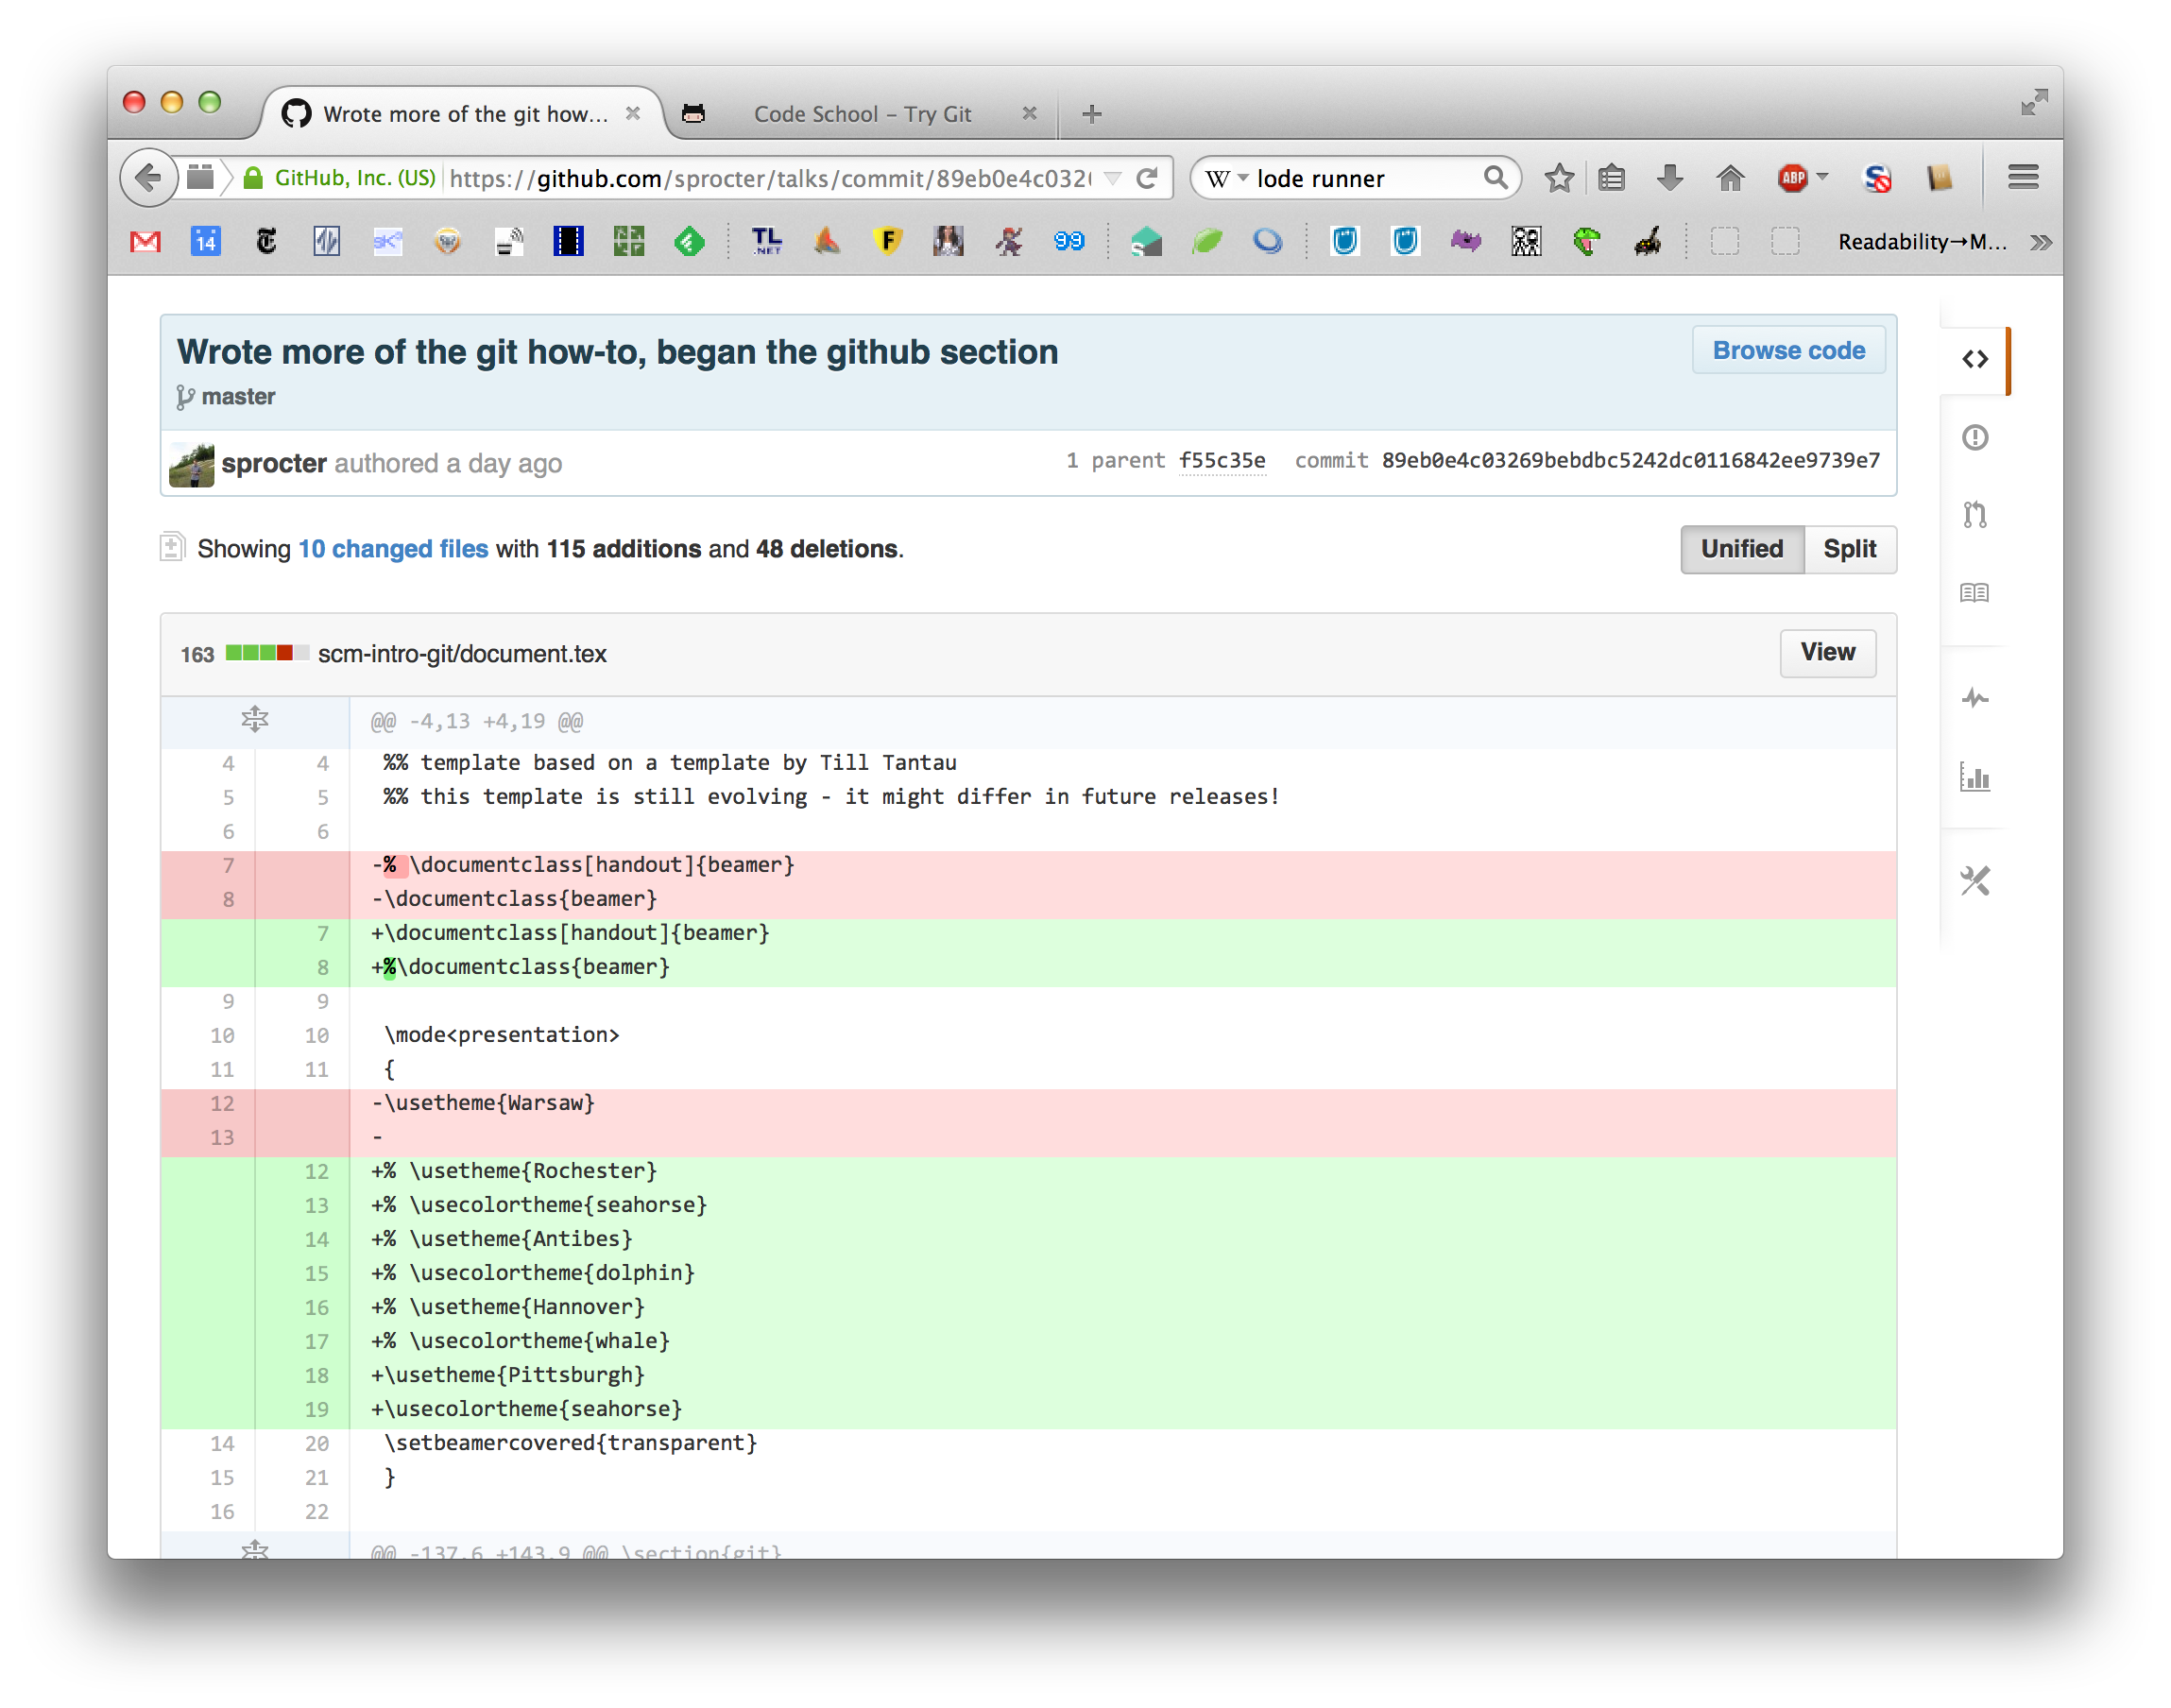
\includegraphics[width=.8\textwidth]{figures/commit-diff}
\end{figure}

\end{frame}

\section{Be Brave!}

\subsection[Learn by playing]{Learn by playing}

\begin{frame}
\frametitle{Be Brave!}
\begin{figure}[!t] \centering

\includegraphics[width=.4\textwidth]{figures/jake-quote}
\end{figure}
\begin{itemize}
\item git is \emph{tremendously} googlable.
\item Breaking things (especially after a commit / push) is very difficult
\item Play with it!
\end{itemize}
\uncover<2->{No seriously, try it right now with either:
\begin{itemize}
\item \alert{https://try.github.io}
\item Your own github account
\end{itemize}}
\end{frame}

\begin{frame}[allowframebreaks]
  \frametitle<presentation>{References}    
  \begin{thebibliography}{10}    
  \beamertemplatebookbibitems
  \bibitem{sink:BOOK2011}
    Eric Sink.
    \newblock {\em Version control by example}.
    \newblock Pyrenean Gold Press, 2011.
  \bibitem{sink:BOOK2011}
    Scott Chacon.
    \newblock {\em Pro Git}.
    \newblock Apress, 2009.
%   \beamer
  \beamertemplatearticlebibitems
  \bibitem{github-help}
    Github, Inc.
    \newblock \url{https://help.github.com}
%     \newblock {\em Journal of This and That}, 2(1):50--100, 2000.
  \end{thebibliography}
\end{frame}
\end{document}
